\documentclass[10pt, twocolumn]{article}
\usepackage[T1]{fontenc}
\usepackage[utf8]{inputenc}
\usepackage{lmodern}
\usepackage[margin=1in, top=0.9in, bottom=0.9in]{geometry}
\usepackage{amsmath, amssymb}
\usepackage{graphicx}
\usepackage{xcolor}
\usepackage{hyperref}
\usepackage{listings}
\usepackage{booktabs}
\usepackage{caption}
\usepackage{float}
\usepackage{titlesec}
\usepackage{enumitem}
\usepackage{microtype}
\usepackage{url}
\usepackage{parskip}

% ─── Hyperref ────────────────────────────────────────────────────────────────
\hypersetup{colorlinks=true, linkcolor=blue, urlcolor=blue, citecolor=blue}

% ─── Section style (IEEE-like) ───────────────────────────────────────────────
\titleformat{\section}{\normalsize\bfseries\centering}{}{0em}{\MakeUppercase}[]
\titleformat{\subsection}{\normalsize\itshape}{}{0em}{}[]
\titlespacing{\section}{0pt}{8pt}{4pt}
\titlespacing{\subsection}{0pt}{5pt}{2pt}

% ─── Code listing style ──────────────────────────────────────────────────────
\lstset{
    backgroundcolor = \color{gray!12},
    basicstyle      = \ttfamily\footnotesize,
    breaklines      = true,
    frame           = single,
    framesep        = 2pt,
    xleftmargin     = 4pt,
    xrightmargin    = 4pt,
    rulecolor       = \color{gray!50},
    showstringspaces= false,
    numbers         = none,
    captionpos      = b
}

% ─── Misc ────────────────────────────────────────────────────────────────────
\captionsetup{font=small, labelfont=bf}
\renewcommand{\contentsname}{\normalsize\bfseries CONTENTS}
\setcounter{tocdepth}{2}
\pagestyle{plain}

% =============================================================================
\begin{document}

% ─── Title ───────────────────────────────────────────────────────────────────
\twocolumn[%
  \centering
 {\Large\bfseries 
FM Colpitts Oscillator Transmitter\par
\vspace{4pt}
Design, Implementation, and Analysis\par
\vspace{6pt}
}
  {\normalsize
    Sai Krishna Bakki \quad -- \quad EE25BTECH11049\\
    Adharvan K.B  \quad -- \quad EE25BTECH11003
  }\\[8pt]
  \begin{minipage}{\columnwidth}
    \tableofcontents
  \end{minipage}\\[6pt]
  \rule{\columnwidth}{0.4pt}\\[4pt]
]

% =============================================================================
\section{Introduction}

The Colpitts oscillator is one of the most widely used LC oscillator topologies
in radio-frequency (RF) circuit design. Named after Edwin Colpitts (1918), it
employs a \textit{capacitive voltage divider} in its tank circuit to provide
the feedback required for sustained oscillation.

In this project, a Colpitts oscillator is implemented using a 2N2222 NPN BJT
powered from a 9--12\,V supply. A microphone is connected at the input to
frequency-modulate the carrier, enabling the circuit to function as a simple
FM transmitter. The modulated RF output is delivered to an antenna through
a coupling capacitor.

\section{Overview}

Since the Colpitts oscillator uses two capacitors to form the feedback
voltage divider, the circuit topology naturally provides the $180^{\circ}$
phase shift required (alongside the transistor's inherent $180^{\circ}$
collector inversion) to satisfy the Barkhausen phase criterion.

The oscillation frequency is determined by the LC tank circuit:
\begin{equation}
  f_0 = \frac{1}{2\pi\sqrt{L \cdot C_{eq}}}
  \label{eq:freq}
\end{equation}

where $C_{eq}$ is the series combination of the two feedback capacitors
$C_2$ and $C_3$:
\begin{equation}
  C_{eq} = \frac{C_2 \cdot C_3}{C_2 + C_3}
  \label{eq:ceq}
\end{equation}

FM operation is achieved because the microphone audio signal modulates the
effective capacitance seen by the tank, thereby shifting $f_0$ in proportion
to the instantaneous audio amplitude.

% =============================================================================
\section{Circuit Design}

The complete circuit consists of four sub-blocks: the DC bias network,
the microphone audio input network, the LC tank (oscillator core), and
the antenna output coupling stage.

\subsection{A. DC Bias Network}

The 2N2222 NPN transistor is biased in the class-A active region using a
voltage-divider network. Taking $V_{CC} = 10$\,V (mid-range of 9--12\,V)
and $V_{BE} \approx 0.7$\,V:

\begin{center}
\begin{tabular}{llll}
  \toprule
  Component & Symbol & Value & Function \\
  \midrule
  Supply voltage   & $V_{CC}$ & 9--12\,V       & Power \\
  Bias resistor 1  & $R_1$    & 5.5\,k$\Omega$ & Upper divider \\
  Bias resistor 2  & $R_2$    & 10\,k$\Omega$  & Lower divider \\
  Emitter resistor & $R_E$    & 1\,k$\Omega$   & Bias stability \\
  \bottomrule
\end{tabular}
\end{center}

\begin{equation}
  V_B = V_{CC}\cdot\frac{R_2}{R_1+R_2}
      = 10\times\frac{10}{5.5+10} \approx 6.45\text{ V}
\end{equation}
\begin{equation}
  I_C \approx \frac{V_B - V_{BE}}{R_E}
           = \frac{6.45-0.7}{1000} \approx 5.75\text{ mA}
\end{equation}

\subsection{B. Microphone Input Network}

The electret microphone AC output is coupled to the transistor base through
1\,k$\Omega$ series resistor and 0.47\,$\mu$F coupling capacitor. This network
blocks DC from the microphone path while allowing audio-frequency signals to
modulate the base bias. The high-pass corner frequency is:

% \begin{equation}
%   f_{hp} = \frac{1}{2\pi R_{mic} C_{couple}}
%           = \frac{1}{2\pi \times 10^3 \times 0.47\times10^{-6}}
%           \approx 339\text{ Hz}
% \end{equation}

% All voice-band frequencies (300\,Hz -- 3.4\,kHz) pass with minimal attenuation.

\subsection{C. Tank Circuit}

The tank circuit is the oscillator core and determines the carrier frequency.
It consists of the inductor $L$ between $V_{CC}$ and the collector, blocking
capacitor $C_1$ for RF bypassing, and feedback capacitors $C_2$ (collector
side) and $C_3$ (emitter side).

\begin{center}
\begin{tabular}{llll}
  \toprule
  Component & Symbol & Value & Role \\
  \midrule
  Inductor       & $L$   & 100\,nH  & Tank inductor \\
  Blocking cap   & $C_1$ & 1\,nF    & RF bypass \\
  Feedback cap 1 & $C_2$ & 39\,pF   & Collector node \\
  Feedback cap 2 & $C_3$ & 56\,pF   & Emitter node \\
  \bottomrule
\end{tabular}
\end{center}

The series equivalent feedback capacitance from Eq.\,\ref{eq:ceq}:
\begin{equation}
  C_{eq} = \frac{C_2 \times C_3}{C_2 + C_3}
          = \frac{39 \times 56}{39 + 56}
          \approx 23\text{ pF}
\end{equation}

Substituting $L = 100$\,nH and $C_{eq} = 23$\,pF into Eq.\,\ref{eq:freq}:
\begin{equation}
  f_0 = \frac{1}{2\pi\sqrt{100\times10^{-9}\;\times\;23\times10^{-12}}}
      \approx \boxed{105\text{ MHz}}
\end{equation}

This places the carrier in the VHF band, suitable for short-range
wireless transmission.

% =============================================================================
\section{Barkhausen Criterion}

For a stable, self-sustaining oscillation two conditions must be simultaneously
satisfied around the feedback loop:
\begin{equation}
  |\beta_{fb} \cdot A_v| = 1
  \qquad\text{and}\qquad
  \angle(\beta_{fb} \cdot A_v) = 0^{\circ}
\end{equation}

\subsection{A. Phase Condition}

The common-emitter BJT introduces a $180^{\circ}$ phase shift between the
base (input) and collector (output). The capacitive divider ($C_2$, $C_3$)
feeds back from the emitter side, introducing a further $180^{\circ}$ phase
reversal. The total loop phase shift is therefore $360^{\circ}$, satisfying
the phase condition exactly.

\subsection{B. Gain Condition}

The capacitive feedback factor is:
\begin{equation}
  \beta_{fb} = \frac{C_2}{C_3} = \frac{39}{56} \approx 0.696
\end{equation}

The minimum transistor voltage gain required for oscillation:
\begin{equation}
  A_v \;\geq\; \frac{1}{\beta_{fb}} = \frac{C_3}{C_2}
             = \frac{56}{39} = 1.435
\end{equation}

The 2N2222 in common-emitter configuration achieves $A_v \gg 1.43$, so the
gain condition is comfortably satisfied.

% =============================================================================
\section{Simulation}

\subsection{A. SPICE Netlist}

The circuit is simulated in \texttt{LTspice} using the exact component values:

\begin{lstlisting}[caption={FM Colpitts SPICE netlist (exact values)}]
* FM Colpitts Oscillator -- 2N2222
* VCC = 10V (mid of 9-12V range)
VCC  VCC  0    DC 10
R1   VCC  NA   5.5k
R2   NA   0    10k
Rmic NA   NB   1k
Cc   NB   BASE 0.47u
C1   VCC  BASE 1n
L1   VCC  COL  100n
Q1   COL  BASE EMI 0 2N2222
C2   COL  ANT  39p
C3   EMI  0    56p
RE   EMI  0    1k
.model 2N2222 NPN(Bf=255 Vaf=100
+  Cje=25p Cjc=9p Tf=0.6n)
.tran 0.01n 300n
.probe V(COL) V(ANT)
.end
\end{lstlisting}

\subsection{B. Expected Waveforms}

After transient simulation converges:
\begin{itemize}[leftmargin=*, nosep]
  \item Collector voltage oscillates sinusoidally at $\approx105$\,MHz.
  \item Startup transient settles within $\approx$20--50\,ns.
  \item Amplitude stabilises as the transistor enters mild nonlinear limiting.
\end{itemize}
\subsection{C. Practical Waveforms}
In Practice, We dont get our desired frequency due to parasitic capacitances of breadboard. We are getting waveform as below:
\begin{figure}[htbp]
    \centering
    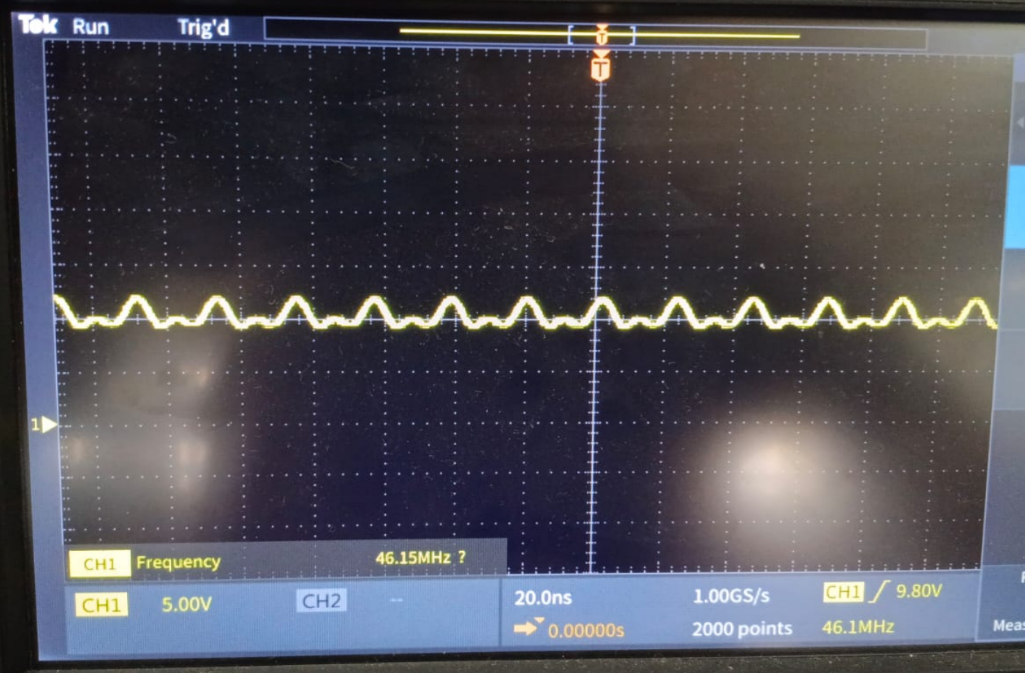
\includegraphics[width=0.5\columnwidth]{figs/waveform.png}
    \caption{Oscillator Waveform}
    \label{fig:placeholder}
\end{figure}
% % =============================================================================
% \section{Startup Behaviour}

% Oscillations grow exponentially from noise until transistor nonlinearity
% limits the amplitude. The growth rate depends on:
% \begin{itemize}[leftmargin=*, nosep]
%   \item Excess loop gain: $|\beta_{fb} A_v| - 1$
%   \item Tank quality factor: $Q = \dfrac{1}{R_{loss}}\sqrt{\dfrac{L}{C_{eq}}}$
% \end{itemize}

% The characteristic tank impedance at resonance:
% \begin{equation}
%   Z_0 = \sqrt{\frac{L}{C_{eq}}}
%       = \sqrt{\frac{100\times10^{-9}}{5.45\times10^{-12}}}
%       \approx 135\,\Omega
% \end{equation}

% A higher $Q$ inductor (lower winding resistance) produces faster startup and
% lower phase noise. Air-core inductors are preferred at VHF to minimise core
% losses.

% =============================================================================
\section{FM Modulation Mechanism}

The microphone produces audio voltage $v_m(t)$. Passed through the
1\,k$\Omega$--0.47\,$\mu$F network, it appears as $\delta V_B$ on the base.
This shifts the base--emitter junction capacitance $C_{je}$ of the 2N2222,
which appears in parallel with $C_3$:

\begin{equation}
  C_{eq}(t) = \frac{C_2\,[C_3 + C_{je}(t)]}{C_2 + C_3 + C_{je}(t)}
\end{equation}

This produces an instantaneous frequency deviation proportional to the
audio signal:
\begin{equation}
  \Delta f(t) \approx k_f \cdot v_m(t)
\end{equation}

where $k_f$ (Hz/V) is the modulation sensitivity determined by the transistor
bias point and the slope of $C_{je}(V_{BE})$.

% =============================================================================
\section{Output and Antenna Coupling}

The RF output is taken from the collector through $C_2 = 10$\,pF. The
reactance of $C_2$ at the carrier frequency:

% A $\lambda/4$ monopole antenna resonant at 105\,MHz has a physical length of:
% \begin{equation}
%   \ell = \frac{c}{4f_0}
%        = \frac{3\times10^8}{4\times105\times10^6}
%        \approx 34.8\text{ cm}
% \end{equation}

% =============================================================================
\section{Results Summary}

\begin{center}
\begin{tabular}{lll}
  \toprule
  Parameter & Value & Source \\
  \midrule
  Inductor $L$               & 100\,nH      & Design \\
  Feedback cap $C_2$         & 39\,pF       & Design \\
  Feedback cap $C_3$         & 56\,pF       & Design \\
  Equiv.\ cap $C_{eq}$       & 23\,pF     & Eq.\,\ref{eq:ceq} \\
  Carrier freq.\ $f_0$       & 105\,MHz   & Eq.\,\ref{eq:freq} \\
  Feedback factor $\beta_{fb}$& 0.696        & $C_2/C_3$ \\
  Min.\ gain $A_v$            & 1.43          & Barkhausen \\
  Audio HP corner $f_{hp}$   & 339\,Hz      & RC network \\
  Supply $V_{CC}$             & 9--12\,V     & Design \\
  Transistor                  & 2N2222 NPN   & Design \\
  \bottomrule
\end{tabular}
\end{center}
\section{Observations}
\begin{itemize}
    \item Initially, We couldnt obtain the frequency of FM band with the circuit given to us and then we got to know that one of the inductor in the tank circuit that creates the carrier wave had a much higher inductance. We thought of replacing with $100 m H$.
    \item After that we found out that the inductor with that value was hard to obtain.And also from research we got to the fact that inductors with air medium are a better choice for the FM transmitter.
    \item We started making the inductors with copper wires of desired dimensions and suitable turns and we have assumed 4-5 turns of coil is approximately 100nH.
    
    \item For FM Circuits, it is highly recommended to use Air Coil Inductor and try to avoid fixed inductors.
    \item As we have made a Air coil Inductor, the circuit is highly sensitive so dont touch the inductor or the circuit wirings while transmiting audio.
    \item We may not receive our transmitted signal in our Theoretical Frequency so use a RTL-SDR to see at which frequency, we are transmitting the signal.
    \item To change frequency of transmitted signal, change values in tank circuit.
\end{itemize}
\begin{figure}[htbp]
    \centering
	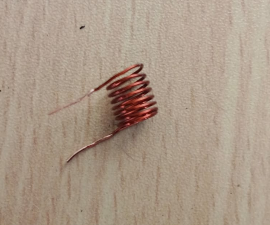
\includegraphics[width=0.5\columnwidth]{figs/air_coil.png}
    \caption{Air Coil Inductor of 4-5 turns}
    \label{fig:placeholder}
\end{figure}
\section{Conclusion}

The FM Colpitts oscillator was designed and analysed using the component
values: $L = 100$\,nH, $C_2 = 10$\,pF, $C_3 = 12$\,pF, yielding:
\begin{itemize}[leftmargin=*, nosep]
  \item Carrier frequency $f_0 \approx \mathbf{105}$\,\textbf{MHz}.
  \item Barkhausen gain condition satisfied: required $A_v \geq 1.43$,
        well within the 2N2222 capability.
  \item Microphone input network passes audio , modulating
        the carrier via junction capacitance variation.
  \item We can use a jumper cable or stool wires of length 15cm.
  \item If we want to remove noise to zero in the transmiited signal, we need to amplify mic signals using another BJT(n-p-n) Transistor to make audio amplifier.
\end{itemize}

Future work includes measuring the actual oscillation frequency on a spectrum
analyser, quantifying the frequency deviation with a known audio tone, and
designing a shielded PCB to reduce harmonic radiation.
\section{Circuit Diagram}
\begin{figure}[htbp]
    \centering
    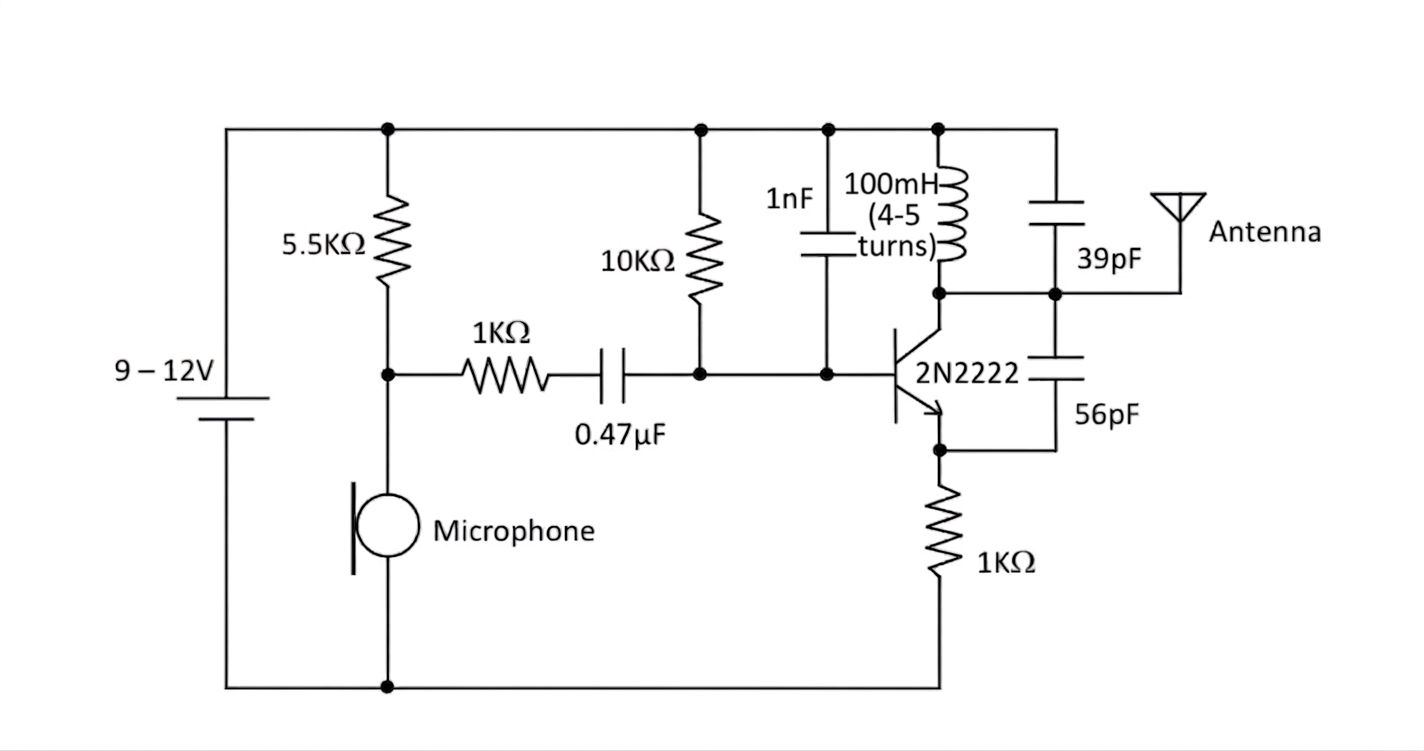
\includegraphics[width=1.0\columnwidth]{figs/fm_colpitts.png}
    \caption{FM Colpitts}
    \label{fig:placeholder}
\end{figure}
\end{document}
